\section{Visual exploration of data}
\begin{frame}
    \frametitle{An introduction to PowerBI}
\begin{block}{A report generator}
    \begin{itemize}
        \item<+-> Power BI is a reporting and data analytics tool.
        that simplifies data collection, transformation, 
        and visualization tasks.
        \item<+-> It is designed to be extensible and tends has become
        the de facto standard in the industry.
    \end{itemize}
\end{block}
\begin{block}{What PowerBI is not}
    \begin{itemize}
        \item<+-> While it performs well in terms of data visualization,
         it is not a full-fledged statistical software.
        \item<+-> The use of a superior data transformation
         and analysis tool is a highly effective strategy.
    \end{itemize}
\end{block}    i
\end{frame}
\begin{frame}
    \frametitle{R}
\begin{block}{The workhorse of statistics}
    \begin{itemize}
        \item<+-> A free and open source piece of software.
        \item<+->R boasts implementation of nearly all developments in statistics.
        \item<+-> The number of free programs written in R is keeping increasing.
    \end{itemize}
\end{block}
\begin{block}{A companion to PowerBI}
    \begin{itemize}
        \item<+-> PowerBI can collect data from a R script.
        \item<+-> PowerBI can transform data using a R script.
        \item<+-> PowerBI can display the output of a R script. 
    \end{itemize}
\end{block}    
\end{frame}
\begin{frame}
    \frametitle{R in a nutshell}
\begin{block}{R as a desk calculator}
    \begin{itemize}
        \item<+-> Open R by double-clicking on the R icon.
        \item<+-> Simply type "2+3" and observe the result.
        \begin{figure}[htbp]
            \centering
            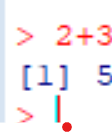
\includegraphics[scale=0.5]{R-sum.png}
            \caption{A simple sum}
            \label{<label>}
        \end{figure}
        \item<+-> A value  can be stored in
        a variable with the operator \texttt{<-}.
        \begin{figure}[htbp]
            \centering
            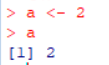
\includegraphics[scale=0.5]{variable.PNG}
            \caption{Using a variable.}
            \label{fig:variable}
        \end{figure}
    \end{itemize}
\end{block}
\end{frame}
\begin{frame}
    \frametitle{Vectors}
\begin{block}{Vectors}
    \begin{itemize}
        \item<+-> Vectors are created using the "c" (concatenate) or range operator "min:max".
        \item<+-> Try "c(0.1, 2, 3)" and "1:100".
        \item<+-> If you want a non-unit step, use the "seq(min, max, step)" command.
        \begin{figure}[htbp]
            \centering
            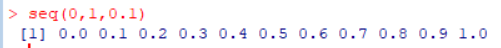
\includegraphics[scale=0.5]{seq_example.png}
            \caption{User-defined step}
            \label{fig:arbitrary_range}
        \end{figure}
        \item<+-> All the elements of a vector must be of the same type:
        numeric (double, integer, complex), logical, string.
    \end{itemize}
\end{block}
\end{frame}
\begin{frame}
    \frametitle{Vectors}
    \begin{block}{Numeric and boolean types}
        \begin{itemize}
            \item<+-> By default, a numeric value is encoded 
            as a double precision number on 64 bits. 
            \item<+-> A complex number is declared with syntax $x + yi$:
           \begin{figure}[htbp]
            \centering
            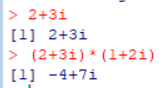
\includegraphics[scale=0.5]{complex_number.PNG}
            \caption{Complex numbers}
            \label{fig:complex_numbers}
           \end{figure}
           \item<+-> Booleans are TRUE or FALSE.
           \begin{figure}[htbp]
            \centering
            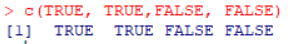
\includegraphics[scale=0.5]{boolean.PNG}
            \caption{Booleans}
            \label{fig:booleans}
           \end{figure}
        \end{itemize}
    \end{block}
\end{frame}
\begin{frame}
    \frametitle{Vectors}
    \begin{block}{Character strings}
        \begin{itemize}
           \item<+-> A string is enclosed with double or simple quotes.
           \begin{figure}[htbp]
            \centering
           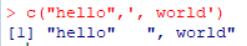
\includegraphics[scale=0.5]{string.PNG} 
            \caption{Character strings}
            \label{fig:char_strings}
           \end{figure}
           \item<+-> Any R object can be converted to an informative string with the function
           \texttt{str().}
        \begin{figure}[htbp]
            \centering
           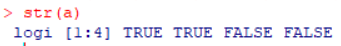
\includegraphics[scale=0.5]{str_func.PNG} 
            \caption{Str function.}
            \label{fig:str_func}
           \end{figure}
        \end{itemize}
    \end{block}
\end{frame}

\begin{frame}
    \frametitle{Vectors}
\begin{block}{Operators}
   \begin{itemize}
    \item<+->Operators and functions are applied elementwise.
     \begin{figure}[htbp]
            \centering
           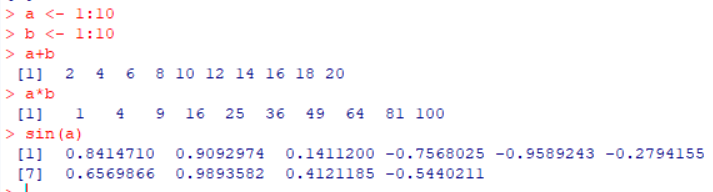
\includegraphics[scale=0.5]{vector_functions.PNG} 
            \caption{Operating on vectors.}
            \label{fig:vect_op}
           \end{figure}
    \item<+-> This is true also for comparison operators.
     \begin{figure}[htbp]
            \centering
           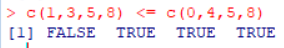
\includegraphics[scale=0.5]{comparison.PNG}
            \caption{Comparison operators.}
            \label{fig:vect_comp}
           \end{figure}
   \end{itemize} 
\end{block}
\end{frame}
\begin{frame}
    \frametitle{Vectors}
    \begin{block}{Accessing elements}
        \begin{itemize}
            \item<+-> An element in a vector can be referred to by its 
            index.
     \begin{figure}[htbp]
            \centering
           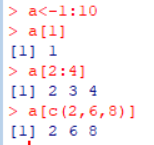
\includegraphics[scale=0.5]{elements.PNG}
            \caption{Accessing elements.}
            \label{fig:vect_elts}
           \end{figure}
           \item<+-> A selection by booleans is also possible.
           \begin{figure}[htbp]
            \centering
           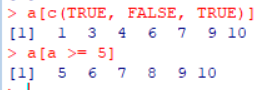
\includegraphics[scale=0.5]{bool_select.PNG}
            \caption{Boolean selection.}
            \label{fig:vect_bool}
           \end{figure}
        \end{itemize}
    \end{block}
\end{frame}
\begin{frame}
    \frametitle{Data frames}
\begin{block}{A convenient object.}
    \begin{itemize}
        \item<+-> Data frames are arrays holding observed values.
        \item<+-> Observed characteristics are in columns, observations in rows.
        \item<+-> The columns are named and can be referred to by their names.
        \begin{figure}[htbp]
            \centering
           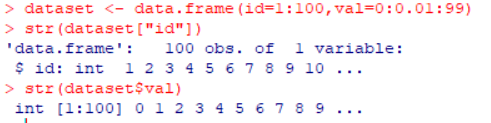
\includegraphics[scale=0.5]{dataframe.PNG}
            \caption{A data frame.}
            \label{fig:data_frame}
           \end{figure}
        \item<+-> Data frames are used by PowerBI to communicate with R.
    \end{itemize}
\end{block}
\end{frame}
